\documentclass[a4paper]{article}
\usepackage{graphicx}
\usepackage{mathtools}
\usepackage[a4paper, total={5in, 6.5in}]{geometry}
\usepackage{color}
\usepackage{tikz}
\usepackage{lipsum}
\usepackage{geometry}
\geometry{a4paper, left=2.5cm, top=2.5cm, bottom=2.5cm, right=2.5cm}
\usepackage{changepage}
\usepackage{booktabs}
\usepackage[font=small]{caption}
\DeclareCaptionFormat{mycaptionfont}{\fontsize{12}{13}\selectfont#1#2#3}
\usepackage{threeparttable}
\usepackage{ntheorem}
\usepackage{caption}
\usepackage{wrapfig,lipsum,booktabs}
\usepackage{listings}
\usepackage{pdflscape}
\captionsetup{format=mycaptionfont}
\usepackage{subcaption}
\theoremseparator{:}
\usepackage{lscape}

\usepackage[utf8]{inputenc}
\newtheorem{hyp}{Hypothesis}
\usetikzlibrary{shapes,decorations,arrows,calc,arrows.meta,fit,positioning}
\tikzset{
    -Latex,auto,node distance =1 cm and 1 cm,semithick,
    state/.style ={ellipse, draw, minimum width = 0.7 cm},
    point/.style = {circle, draw, inner sep=0.04cm,fill,node contents={}},
    bidirected/.style={Latex-Latex,dashed},
    el/.style = {inner sep=2pt, align=left, sloped}
}


\graphicspath{ {/home/angelo/Documents/Uni/Courses/Data Managment & Ethics/Integrated Assignment/assignemnet_project_folder/ERDs/} }


\begin{document}

\title{DME Integrative Assignment}
\author{Angelo Barisano; 508903 }
\date{September 16th, 2022}
\maketitle

\newpage




\section{Task 1: Plan \& Explore}


\textbf{Please note: I try to be precise but sometimes I will not descibe certain features: the fact that a primary key is unique should be given etc. I try to describe everything but sometimes I just have to assume that the correctur knows what this is about. }

\subsection{Origin of Data \& Purpose Introduction}
\paragraph{Introduction} Data drives security. The wide spread adoption of data information systems has been used to recognize crime hot-spots to increase policing efficiency and protect people. Thus, creating effective information systems for crime prevention is at the center of policy makers and executive branches of governments. This trend has led to the Chicago PD reaching out to this data management team with the request of creating a Data Management System for crime-data in Chicago.

\subsection{Purpose of this assignemnt \& data plan}

To this end, a research database will be created in accordance to the FAIR principles (\textbf{Findability, Accessibility, Interoperability, and Reuse}). The expressed goal of this assignment is to offer a database and some fundamental queries for data exploration; i.e. a database with flexible example queries meant to further analysis of the trends discovered in the data. Additionally, any code produced during this endeavour will be made public on GitHub for transparency purposes. 

\paragraph{Data Description in Scope, Volume, and Format}
The data was provided by the Chicago PD contains a sample of 730,900 registered crimes in the administrative districts of Chicago between the years of 2017 and 2021. The initial data source is in CVS-format and pertains to specific recorded crimes in the administrative jurisdiction of the Chicago PD in addition to time, location, crime type, and arrested or not. Thus, the data contact is to be found on the Chicago PD website (\textbf{CITE THE CHICAGO WEBSITE FOR THE DATA}). Considerations regarding the ethical (\& GDPR compliant regardless of whether the data comes from the USA) use of the data will be discussed in part 5 of this assignment. It is notable that, while this data is only a subsample of the total database crime data recorded in this timeframe, the overall trends in the data are still maintained. Thus, the EDA for which this database can be used for further analysing trends uncovered during this assignment. 

\paragraph{Project time frame, researchers, and misc information} The set project time frame is the 27th of August 2022 till 2nd of October 2022. Involved in this project is only one student, Angelo Barisano. Additionally, this project is designed to comply with FAIR standards (\textbf{CITE FAIR STUFF HERE}).


\textbf{ETHICAL CONSIDERATIONS, FAIR, AND GDPR COMPLIANCE?!?!!?}



\subsection{Research Question}

\textbf{MENTION RESOURCE INTENSTIVE CRIMES AS RELEVANT AS WELL IN THE QUESTION (POSSIBLE/ COMMON SUBSECTION STRATEGY USED IN EDA}

\textbf{In an iterative (agile) development cylce the following questions have been set up: Chicago is known for its high homicide rate; this leads to policy makers focusing on this issue the most. }

Upon conducting an initial Exploratory Data Analysis (EDA), three major categories were identified in the data: 

\begin{itemize}
  \item Location
  \item Crime type
  \item Crime record data (time, arrest, etc.)
\end{itemize}

Based on the data categories and EDA, the following research questions guide the creation of the database in increasing complexity. It may be noted, that the questions are ment to not be exact in their nature, but that the purpose of the assignmnet, database, and questions posed are of an explorative nature, evolving while answering said questions. Thus, this assignment is interpreted as an initial exploratory data analysis meant to uncover trends for further analysis in addition offering useful insights to polciy makers. 

\paragraph{Question 1} Finding prevalent crime patterns in the data is a common starting point in exploring crime data. Crime trends take the form of temporal patterns distributed over a defined timeframe of interest. This kind of reporting is commonly used by policy makers (such as atourney generals) who are monitored based on their performance in terms of crime prevention and the overall trend that can be observed. 

Thus, this question provides future research with an adjustable query to gain an overview over the general distribution of crime by type. Subsequently applying a temporal component (i.e. by day of week,  month, year, season, etc.) to this initial distribution reveals trends and temporal patters. This way, this question helps to answer questions to policy makers regarding general trends; such as how crime developed overall and by type. 

More importantly, however, is that the descriptive analysis of temporal patterns may indicate areas of interest that may be examined more closely by further questions (Q2 \& Q3) through its explorative lense. As such:

\begin{itemize}
  \item What are the overall crime trends that can be observed in Chicago between 2017 and 2021? What crime types changed a lot? 
    \item Primarily: Find interesting crimes in the data for further analysis in Q2.
\end{itemize}





In order to keep the report in a reasonable frame, a primary focus will be laid on \textbf{WHAT??}

This question will be answered by usding a view which contains the date per crime in a convenient manner, such as year, month, day, hour. This way, the analysis is decreased in complexity; providing future researchers with easy to use time dimensions. Moreover, in this question, a variety of window function will be used to group by the time dimension and return a distribution per time component (eg year).

\paragraph{Question 2} The next logical progression is to observe the location and crime dimension together. Certain crime trends, such as those of homicides, may be more localized; thus, certain neighborhoods and districts may be overrepresented in heavy crimes. The assumption is that certain districts and beats tend to be more prevalent in certain crime types. As such, in order to help the PD and policy makers to identify probelmatic areas with respect to certain crime hotspots, districts and beats are analysed with respect to trends identified by the temporal compornent on a localized level. Thus, question two follows:

\begin{itemize}
  \item Based on overall trends discerned in question 1, what locations (beats \& districts) are disproportinally represented overall and in selected subcategories of crimes (based on Q1)?
  \item Primarily: Find districts and beats to disect by time of day and also look into categories of murder in Q3
\end{itemize}

This question will be answered similarly as Q1. However, the main focus here is laid on using standard $GROUP BY$ functions instead of window functions to demonstrate a variation in usage. 

\paragraph{Question 3} Finally, time, location, and crime type is triangulated. This enables policymakers to discern localized trends in the data in order to address crime patterns by distributing resources more efficiently; i.e. allocating more resources to dangerous beats during the night. Additionally, accessory dimensions will be integrated into the analysis to provide a holistic description. For instance assuming that crimes that lead to more arrests are more resource intensive, these crimes put a disproportionate strain on law enforcement. Thus, by triangulating arrests by location and e.g. time of day this will enable us to show areas that need more attention by law enforcement. Another angle would be a specific analysis of beats. \textbf{Beats are the smallest administrative unit of a police district; a beat is patrolled for one year by one unit and ten transferred to another beat. Thus, it might be interesting to investigate the connection between a subset of beats that suddenly stop showing problems during one year and then re-appear in terms of crime in another year. The sub-question would, thus, investigate whether beats that usually persisted in crime only persist on a closed yearly basis. This way, effective police units might be identified and resources might be allocated more efficiently.}
 
\begin{itemize}
  \item Triangulating time, crime-type, and location which areas persists in certain crimes wrt. time?
In order to prevent homicides; which “beats“ are the most prevalent among homicides? During which time of day (for effective allocation of policing resources)? 

\textbf{BASED ON THE LOCATION AND THE }
\end{itemize}

As such, the final question considers a variety of hypotheses that can be explored. Overall, these project based questions are constructed in such a way that they guide an external user (PD) through the process of finding areas that need successively complex "sliced \& diced" information and culminate in the creation of actionable policy implications regarding prime prevention through resource allocation.

AS such, by the descriptive and explorative nature of the questions posed, one can deduce that the entire analysis can be conducted using simple SQL functionalities.

\textbf{ADD PLOTS of EDA ALREADY HERE!!!}


\section{Task 2: Design and Organize}
\textbf{IMPORTANT: DISCUSS what 1st and second normal form means that that all entities are in 2nd normal form by default and due to the structure in 3rd nf!!!}


\textbf{IMPORTANT!!!! READ THE DEFINITION FOR 3rd NF AGAIN; MAYBE CRIME AND LOCATION QUALIFY TO BE 3rd NF... but maybe also not. STRESS AGAIN THAT THE INCLUSION OF BLOCK IS NOT NEEDED FOR THIS RESEARCH!!!}

The aforementioned questions in task 1 require three relevant datacategories, as identified in the data. These pertain to the 1) time dimension, 2) location dimension, and 3) the crime or case instance itself. Generally, these already display common characteristics of regular entities in a relational database (\textbf{CITE HERE BOOK FROM BACHELOR COURSE}). Generally, the design of the database followed the approach of combining logical structures (e.g. location) with an easy to use query design to explore the data.

We will start out with the case entity, as cases recorded in the original data create the centerpiece for all three posed questions.



\paragraph{Entity 1: Case} The first component consist of the individual instances of cases. Conceptually, these are central to this project as they enable the creation of the frequency distributions conditional on time and/or location. The variables that define this entity are as follows:

\begin{itemize}
  \item CaseId
  \item DateTime object implicitly containing day, month, year, and time of day 
  \item Arrest Boolean  
\item \textbf{Location Description???????????????????????????????????????????}
\end{itemize}
 
It may be noted that items such as location description and location themselfes, though listed, are not included in the final product in order to comply with the principle of data minimization (\textbf{\textit{CITE GDPR}}. This is also reduces the possibility of mistakes from occuring. 

The DateTime object will enable the clustering of crimes by the time dimension; which will be done via a view. Additionally, arrest information is used to further drill down the analysis and dissect the cases for more resource intensive cases. This is part of discenring interesting trends and exploring the data. The primary use case of case as an entity, however, is to make the entire database 1) work from a logical perspective (no crime distribution without each individual crime) and 2) to be the logical link between the type of crime committed in every case and where it happens. This way, the case entity is not only a natural entity, but it also fulfills the purpose of making the following two dimensions compliant to the 2nd normal form (and to some extend compliant with 3rd normal form with some caveats) by default. Imagine that if we were to leave out case as an entity and immediately match crime types and location, the resulting two entities could not comply with 3rd normal form as crime types and location (as categories) would produce a many-to-many relationship - thus, not minimizing storage space, increasing query diffuclty, and cause an inefficient relational database. As such, the case entity inadvertently functions as an associative entity, reducing many-to-many relationships to two many-to-one relationships.\footnote{I will not further elaborate on this; this is a logical conclusion; in order to reach 2nd normal form this is a required step which is obvious} As a consequence, case complies to the 3rd NF by definition as no stand alone entities are to be found in this entity (i.e. no transitive dependencies as will be described later), while requiring the other data categories to normalize as well.

 It is notable, that while such design choices should be reflected by leaving out case as an entity in the conceptual model in part 3 and then include it as part of the logical model, but case is so pivotal to the functioning of the database in its purpose, that we will consider it along the way a a valid entity.
 
Please note that any datetime object should not get its own entity. This would violate rules set for relational databases \textbf{CITE BACHELOR STUFF HERE} as any instance created for case requires an instance to be creased in a datetime relation; this would make the relation a one to one relationship, which are not efficient from a storage perspective. 
 
Consequently, no problems of resolving many-to-many relationships are imposed on the design (i.a. no normalization issues later), while minizmizing storage usage, in addition to adding an intuitive centerpiece to the database being implemented.  
 
%Finally, the dimensions of Latitude and Longitude will be included on the case level. The reason for this is, while lat-lon information pertains to the location category, this variable(s) is case specific due to its precision. Imagine the database where latitude and longitude would be described as a standalone entity hierarchically below district or beat. To make the relation work each location would have to carry a CaseId as a foreign key in order to identify what type of crime was perpetrated at this location. Assuming that the lat-lon information is sufficiently granular, this would create a one-to-one relationship between case and the lat-lon entity (disregarding district in this case). Any one-to-one relationship is redundant. Thus, it does not make sense to place lat-lon as a standalone entity hierarchically below district. The reason for the inclusion of lat-lon is its usage as geopandas objects in plotting crime in a heat-map in part 6. Please note that while the information of lat-lon technically violates 1st NF requirements, this information is not supposed to be processed via SQL (except for PostGIS applications) but as a datatype in scripting languages; thus it is an atomic item.




\paragraph{Entity 2: Crime Type} Every Case requires a crime to be a valid instance. The raw data provides the IUCR, which identifies each unique combination of primary (e.g. homicide) and secondary crime category (e.g. first degree). Generally, most headlines only consider the primary type of crime, such as homicides, and generally disregard the secondary description of the data, such as first, second, or third degree in this case \textbf{CITE SOME EXAMPLE NEWSPAPERS}. However, for certain crimes, such as homicide, it might be useful to be more differntiated wrt. eg. gang related homicides.it is also the task of a FAIR database to enable future users to differentiate between different types of general crimes. Furthermore, it might be the case, that certain subcategories of crimes tend to be more prevalent than others.
Subsequently, due to the inclusion of the secondary description of the crime, this necessitates that crime type is an entity on its own. Suppose only the primary category of any crime commited was to be analysed. This would imply that both the IUCR and secondary description would be superflous. Subsequetnly, any entity with only one variable is a superflous entity, taking up unnecessary storage space (similar to one to one relationships). The reason for this is that if a crime occurs, a foreign key would have to relate the primary crime type to the crime type entity. Obviously, the primary crime type foreign key would be the only variable (and primary key) in crime type. As such, it would not make sense from a relational perspective to split crime type into a separate entity. It would make more sense to integrate it directly into the case entity. However, now, due to the inclusion of seconday description as an attribute, crime type has to be its own entity in order to move the case table from 2nd to 3rd normal form (the crime type information would not be transitive). Subsequently, the creation of a crime type entity moves both the case entity and crime type entity into 3rd normal form. Moreover, IUCR then becomes a natural PK (and FK) in this relationship. Subsequently, through the initial design choice, any issues regarding normalization are being taken care of. 


\paragraph{Entity 3: Location} Finally, the location information is being considered. Here, a similar logic applies as with the crime type. In order to analyse certain administrative boundaries, such as districts etc., a location entity has to be included. Hypothetically, if we were to only include information in the database pertaining to in which district an instance of a crime was recorded, the aforementioned case entity would be the most optimal place for such a varaible to be stored. However, this research database aims at offering the ability to further analyse certain subsections of particular police districts - their beats in order to offer better descriptive results. 
Subsequently, any instance of a crime recorded will have its district and beat included. Following hierarchically, beats are below district; one district containing multiple beats. This implies that the most optimal database structure is to use beat as the primary and foreign key in this relationship. This way, any normal form issues are resolved by default, setting both the case and location entity into 3rd normal form. 

The reason to exclude block as a entity of analysis is twofold. 1) blocks overlap to some extend with different districts and beats increasing the level of analysis unnecessarily. 2) Beats and districts are administrative units, while blocks require local knowledge, which is what we try to use to answer for the aforementioned questions. 


\paragraph{Logging \& Master Table} Finally, a small master table will be included which tracks any information regarding formatting the data, data retrieval, and restrictions/ triggers called (not included in part 3 due to relevancy). Such relations are not part of the standard relationship model and are, thus, excluded from the ERD development in part 3. 


\paragraph{Conclusion} Based on the questions posed during task 1 in addition to the fundamental nature of the data provided, the structure described in this section offers an intuitive optimal solution for any normal form problems that might arise. Particularly the inclusion of the case enitiy as an inttegral part of the relationship model automatically resolves any issues pertaining to the inclusion of location and crime type information on a case by case level. 



\section{Part 3: ERD}

\

\begin{figure}[htp]
		\centering
		\includegraphics[scale=.40 ]{ConceptualDiagram.drawio.png}
         \small
         \caption{Conceptual Diagram}
\end{figure}



\subsection{Conceptual Model}
As mentioned in part 2, the individual criminal case instance is central to the database design. Contemporaneously, the case entity resolves all problems regarding normal form (all tables are in 3rd NF) and many-to-many relationships. Subsequently, the conceptual model describes the relation of the three entities described in part 2: 

\begin{itemize}
  \item Location
  \item Case
  \item Crime Type
\end{itemize}

\indent Disregarding information regarding keys, the structure outline in part 1 \& 2 is described here from left to right. To start with, the location entity describes where any crime instance is taking place in terms of beat and implictily the corresponding district. Consequently, location is related to criminal case with a one (non-mandatory) to many (mandatory) relationship, red from left to right. 
The reason for this specific choice of cardinality is simple: in order to be included in the data, a district or beat must have had at least one crime happening in it; otherwise it would not show up in the raw data. As we are not creating a true transactional database, but rather a research project database, we do not have to care for the hypothetical case of a district being included just to make sure you can create future crime isntances in this specific location instance. In order to be included in the raw data, a location (be it beat or district) must have experienced at least one crime instance. Thus, for this specific case of a research project driven database, the $model$ is requiring any location to have at least one crime isntance. A similar arugment will be used further down as well. Contrarily, certain crimes do not have a location; think of fincancial crimes. It would be wrong to remove these records. Thus, a criminal case instance does not need a location.

\indent As such this is then read as: one location must have experienced at least one or many criminal cases; One crimninal case can occur in one and only one, but not mandatory, location instance.

\indent Subsequently, we need the criminal case entity, which contains all case related information on an individual subject basis. Continuing to the right of it, case and crime type is related via a mandatory one or many and mandatory one and only one relationship. Crime type gives the general description to each criminal case (description is the same as in part 1 and 2). The choice for this cardinality is similar to the aforementioned relationship. A criminal case must have a crime type, otherwise it is invalid as no crime would have been committed. Contrarily, a crime type, in order to be included in the initial raw data, must have been committed once at least. This is actually the case here. Certain IUCRs, which exist in the penal code in Ilinois, were not committed and are thus not included in the raw datafile.

\indent As such this is then read as: one criminal case pertains to one (mandatory) and only one crime type; one crime type can be perpetrated in one or many (mandatory) criminal cases.


\paragraph{Intermezzo:} It may be notable that the model shows mandatory relationships for crime type and location. Technically correct would be to use non mandatory relationships for location and crime type. For example a district or crime may not have been perpetrated and, thus, would not have a record. This research does not consider this case as the goal of this data base is to use the existing data for analysis. As such, in order for a district/ crime to be included in the database, a crime instance must have been created for these instances. As such, the choice was made to include a mandatory relationship for these cardinalities.

\subsection{Logical Model}


\begin{figure}[htp]
		\centering
		\includegraphics[scale=.40 ]{LogicalDiagram.drawio.png}
         \small
         \caption{Logical Diagram}
\end{figure}

Figure 2 describes the logical model. For location, "beat" is chosen as primary key because beat (as a stand alone entity) would be hierarchically below District; one district - many beats. As such, each district is uniquely identifiable by its beat in case we want to aggregate, which is why beat is the only natural (primary) key in this relation. In realtiy (with more variables in location) this relation is not in 3rd normal form as district is usually an entity on its own. However, due to no more data/ variables being available on beat or district, this relation does not contain any transitive dependencies and is, thus, in 3rd NF. The meaning of each attribute here is selfexplanatory.More importantly, the primary key beat is in TEXT form (also district). The reason for this is that beats are defined in the first two characters by their district and the latter two describe the beat. Thus, a beat instance may start with a "0". In many scripting languages and some databases, this leads to problems and the removal of the "0", as the underlying software does not interpret the "0". As such, TEXT was chosen for data quality reasons. Please note that the same argument applies to crime type and IUCR. 

\indent Following, CrimeID was chosen to be the primary key of case, due to it being a natural primary key. This is a standard auto-incremental integer key and can, thus, be treated as an integer; though care should be applied when reading the data into scripting languages. In addition to each CrimeID identifying each instance of a crime comitted, DateTime and Arrest are included as attributes. DateTime has TEXT as dtype as SQLite does not support a conventional datetime object, which then defaults to a string value. DateTime provides year, month, day, hour, minute, second of the instance 8as any other datetime dtype does by definition). Arrest has the dtype TEXT for a similar reason; SQLite does not support boolean dtypes. A possible alternative would have been to use 1 or 0, but a simple string input TRUE or FALSE has the same functionality in the and while being more explicit. Arrest describes the state of each criminal case whether or not an arrest was made. 


\indent Finally, crime type's primary key is the IUCR key, a natural primary key. It uniquely identifies each crime category plus its secondary description. Its dtype is TEXT for the same reason as for why beat's dtype is TEXT. Following, primary category has dtype TEXT and ´describes the overall category of the crime committed. Secondary category then fruther describes each primary category; thus, it also has a TEXT dtype. 



\subsection{Physical Model}


\begin{figure}[htp]
		\centering
			\includegraphics[scale=.40 ]{PhyscialDiagram.drawio.png}
         \small
         \caption{Physical Diagram}
\end{figure}

As mentioned in part 2, the inclusion of case as a full entity throught the entire process automatically removes any many-to-many relationships. Additionally, this simplified the choice in appropriate foreign keys to describe the relationships. Remember, foreign keys must be placed in the adjacent entity on the many side (the other way around would be counterproductive). Thus, beat is the foreign key in criminal case for location and IUCR is the foreign key in criminal case for crime type. The reason for this should be selfexplanatory. It may be noted that CrimeID is still the unique identifier in criminal case as it is unique by its own right. 

Thus, planing in part 1 and 2 simpliefied this part considerably by default. 


\section{Part 4- Data Quality checks and preparation}

In the process of preparing the data to be loaded into the research DB, python was the scripting language of choice. For transaprency reasons (FAIR) the datapreparation file is contained in an adjacent file. 

In order to conduct the data cleaning, the GDPR's dataminization principle was used (the others, though important, are less applicable here \textbf{CITE GDPR HERE}. Dataminimization states that only data that is actively being used and has a purpose of being stored should be included in a database. While this project is based on a public database from the US (so technically GDPR does not apply; particualrly because no individual is identifiable), GDPR still offers guiding principles/standards on how to fair with data. Additionally, dataminimization has a practical usagepoint: less data means fewer errors.\footnote{Please note that I studied the GDPR at UvA and had to work with it; so I can speak from experience.} Thus, not all data in the raw data is included. This also means that considerations regarding FAIR were made (see part 1).  

In order to prepare the data, the \textbf{data triangle was used} (\textbf{CITE THE LECTURE HERE}. 

\textbf{Now to the data: }Generally, the data quality of the provided  raw sample is very good; less than 0.01\% of observations display any anomalies. This is attribuatble to the origin of the data being of administrative nature by public offices.

\indent The operations performed specifically relate to the relevant data for this endeavour mentioned in part 3. Firstly, 3 instances contained no casenumbers. These records were broken overall and were, thus, removed. Secondly, 16 instances missed date. As date is a central to the analysis, these records have to be removed. Moreover, 79 instances had non-correspondent beats and districts. While it would have been possible to impute the missing data based on the block or lat-lon information, one must assume that all location related information wrt. these observations is compromised. Similarly as before, location quality is central to answering the questions in this assignemnt; thus, these instances were removed. Finally, 149 perfectly dupilcated items were removed. 

\indent In terms of data transformations, date was transformed into SQL castable form to run functions on date. Moreover, beat and district instances were repaired wrt. the preceeding "0" filler, creating instances of length four and two respectively. Finally, arrest ("true", "false") was cast into boolean form. 

\indent Regarding non-crucial anomalies, 15 instances miss arrest; but this information is only used for one subquery once, which is why it was kept. Additionally, seven records of casenumbers display noncompliance. However, CaseID is a perfect reflection for this issue. Considering CaseID, set-tests \textbf{(looking for duplicates in a set object)} were made to warrant that no IDs were missing (see appendix) beyond the removed records. Further, one instance of lat-lon showed an extreme outlier which was converted to NaN, due to the beat and district information appearing propperly.\textbf{ All instances with minor porblems were marked, which will} \textbf{be represented in the MasterTable of this project}. It may also be notable that the absence of information is still information; i.e. financial crime might not have a location (refer to part 3 discussion of cardinalities). 

Overall, the consequences of removing these observations is minimal. Of a total of 730900 observations, we were left with 730654 records. 

Finally, considering crime type related data, secondary description and through that IUCR, contained typos, resulting in duplciated values. However, the typos did not change the meaning of the secondary descriptions. As such, a simple merge-right-join was performed to drop all duplicates on that dimension without loosing any data.

\section{Part 5 - Create Tables and Load the Data}
\textbf{IMPORTANT: ADD CASCADE RESTRCITION TO CASE}

Upon implementing the physical ERD into SQL, location and crime type (implemented as crimetype for convenience when quering) the $CREATE TABLE$ command was used. Beat and IUCR were defined as PK using the $PRIMARY KEY$ command. The $UNIQUE$ + $NOT NULL$ constraint are technically not needed due to the designation of these attributes as PK. They were, however, included to be explicit and clear. Moreover, $NOT NULL$ was applied to the district attribute and primary category (implemented as PrimaryCategory for convenience in querying) as these should not be empty. However, secondary category (implemented as SecondaryCategory) in crime type did not need these restrictions as certain primary types may not have a secondary category.

Following, the criminal case relation (implemented as CriminalCase) contained the only $FOREIGN KEY$ restrictions as described in part 3. Considering constrains implemented wrt. the relations (through foreign keys), upon update and deletion, all related instances in the parent table should be removed: i.e. $CASCADE$ update and deletion (one only implemnets these on the foreign keys to signal SQL how to conduct such operations). The reason for this is twofold: 1) in a usual transactional database, such operations should be restricted as no human should have writing access to a specific instance \textbf{CITE BACHELOR BOOK ON THIS}. However, we are dealing with a reasearch project database; as such, it might be the case that it turns out that one district instance should not exist (is eroneous). As such, all "supposed" crimes that happened in this district would have to be removed. That is why cascasde deletion was chose. Finally, a small $CHECK$ was implemented in order to check the time.\footnote{No "if exists" table creation was implemented as this is bad practice.}


\textbf{DESCRIBE THE MASTER TABLE!!!}
Regarding triggers and the master table, SQLite does not support a conventional query log; thus, we had to resort to using standard implementations for triggers (delete, insert, update). 

%https://www.sqlshack.com/learn-sql-sql-triggers/
%https://www.sqlitetutorial.net/sqlite-foreign-key/
%https://www.crewmachine.com/use-mysql-triggers-recording-history/


%CREATE
%[DEFINER = user]
%TRIGGER trigger_name
%trigger_time trigger_event trigger_id
%ON history_table FOR EACH ROW
%trigger_body
%trigger_time { BEFORE | AFTER }
%trigger_event { INSERT | UPDATE | DELETE }


%INSERT INTO history_table SELECT*, ‘update’,
%CURRENT_USER(), now(), null FROM
%main_table WHERE id=OLD.id;

\section{Part 6}

To do: create master table plus some triggers, add the stuff regarding index and use it, then finish q3.

\textbf{It may be noted that we cannot query all possible outcomes}
\textbf{It may be noted that we cannot query all possible outcomes}
\textbf{It may be noted that we cannot query all possible outcomes}
\textbf{It may be noted that we cannot query all possible outcomes}
\textbf{It may be noted that we cannot query all possible outcomes}

Note: the goal of this assignment t odo most if not all data transformation in SQL and let python handle only minor conversions such as into the right dtype object (eg GEOPANDAS)

IMPORTANT! READ DATABASE INTO PYTHON HERE LIKE YOU DID AT VYTAL!!!

Note: Sadly in order to create an index, one cannot use subqueries due to SQLLITE(this feature is present in other versions of SQL tho); as such, the index that increases speed for arrest heavy crimes does not work here. 

\textbf{FOR THE TRIGGER JUST USE DELETE RESTRICT HERE!!}

Please note that many queries, particularly those meant for visualization were read into python immediately (so they use queries to get the results needed and then lets python do the rest). Additionally, the database was not saved directly in the repository due to security concerns (.gitignore). Moreover, no virtual environment was ste up to facilitate the project. Finally, it is notable that in order to answer the questions, multiple different approaches in writing the queries were chosen, ranging from joining subqueries to window functions in order to demonstrate knowledge of all functions. Another reason is that I wanted to try the speed of different styles of code (particualrly teh procedually generated optimization behind window functions).

\subsection{Question 1:}


The first question considered how overall crime patterns are distributed with respect to the temporal component. To this end, a view containing transformed datetime by crime case  outputs was cosntructed as it would be of use throughout this project. This query utilized a subquery which used the $STRFTIME$ string parser to obtain year, month, day, hour from every crime case instance. Subsequently, the $CAST$ function was used to cast hour/ time of day into monring, noon, evening, night buckets per instance, creating a convenient view to analyse different dimensions of time per each crime (see ViewTab).


\paragraph{Part 1} Consequently, the first sub-question considered what the overall trend in crime was per year; i.e. are total crime levels increasing or decreasing? This question is relevant for public officials, which are helt responsible for overall crime levels. 

In order to answer most questions in question 1, a multitude of windowfunctions was used. For this question two queries were produced: 1) Based on the aforementioned view on time, a $GROUP BY$ was performed on year to $COUNT$ all crime instances per year. This query was used as a subquery in a query using a lagging window function in combination with some casting to calculate the change to the previous year. 2) Utilized the same query, but extended it with a $WHERE$ clause to calculate the total change in crimes over the years (see Question 1 tab part 1).

As can be seen in \textbf{Figure 4 a)} overall crime levels reduced durng the observation time-frame of 2017 to 2021. In 2017, the overall level of crimes recorded was at 161304, which gradually reduced to 124558 crimes committed. Overall, this resulted in a reduction of 22.78\% in total crimes recorded. Thus, on a superficial level, crime tends into the right direction. 


\paragraph{Part 2} However, overall crime levels do not consider the severity of the crime committed. In this context, this analysis focuses on resoruce intensive crimes as a subset. This subset was defined by calculating the proportion of attests in this specific overall (primary) category. It was decided due to berviety concerns that if a crime category displayed more than 50\% arrest rate in addition to more than 500 total arrests over the period of the five recorded years (100 per year), that this crime poses a reasonably higher strain on lawenforcement; this is becasue if such a crime occurs, two lawenforcement officers have to respond only to arrest the suspect in question and bring it to jail while not being able to respond to other calls and if they occur not frequently enough they do not pose a strain on lawenforcement. 

In order to achive this, another view was created (resource intense). This view used multiple $JOIN$ statements joining two queries and multiple tables in those subqueries with a $ROUND$ function to calculate the proportion of arrest to total crimes committed per primary category of crime (see view tab). Secondly, this view was used in the primary query for this part, which joined in a subquery on this view in order to subsect the data by the the specification above and then again applied a lag window function over two partitions (primary category and year) to obtain the total crimes committed and percentage change to previous year per primary crime category ordered by year. Overall, of the 34 primary categories defined in the data seven fulfill this classification. \textbf{Figure 4 b)} shows the development over time of these categories. Primarily Narcotics, while increasing initially, Narcotics related crimes dropped by 56.92\%, posing the most frequent category in this category, starting at 6946 in 2017 and dropping to 2992 records. The largest reduction was observed in Prostition related crimes from 438 in 2017 to 53 in 2021, which constitutes a reduction 89.90\%. Finally, the only category that showed an increase in this subcategory was Weapons Violation, which displayed an increase of 93.89\% vom 2814 to 5456 recorded crimes. Overall, resource intensive crimes showed an overall drop of 29.95\% from 15958 to 11178. Combined with the insight that overall crime levels have dropped, this implies that law enforcement is less strained in 2021 than in 2017. It may be noted that the final drop may be explained by the outbreak of the Corona Virus.

\paragraph{Part 3} When considering all crime categories again, the question which categories, regardless of whether they are resource intensive or not, have shown the largest rise and reduction my be considered. This was achived by utilizing all aforementioned queries and time view in two large queries which used a window function to $DENSE_RANK()$ crimes by the total change over the entire timeframe $LIMIT$(ing) the output once to the five crimes with the largest decrease and once to the five crimes with the largest increase (see tab Question 1 part 3). \textbf{Figure 4 c)} displays the top five categories with the largest reduction, while \textbf{Figure 4 d)} shows those categories with the largest increase in records. While the overall trend was positive in terms of over crime levels reducing, crime categories such as Homicide and Human Trafficing show a 19.94\% and 80.0\% increase respectively. This implies, that while the overall trend in the crime is positive, certain subcategories display a severe increase.  


\begin{wrapfigure}{L}{9cm}
\centering
\begin{subfigure}[b]{0.5\textwidth}
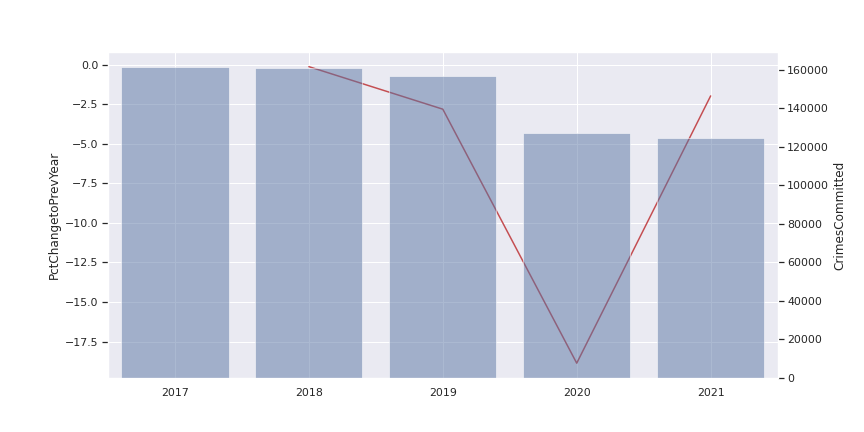
\includegraphics[scale=.3 ]{/home/angelo/Documents/Uni/Courses/Data Managment & Ethics/Integrated Assignment/assignemnet_project_folder/Code/q1_part1.png}
   \caption{Total Crimes Recorded}
   \label{fig:Ng2}
\end{subfigure}

\begin{subfigure}[b]{0.5\textwidth}
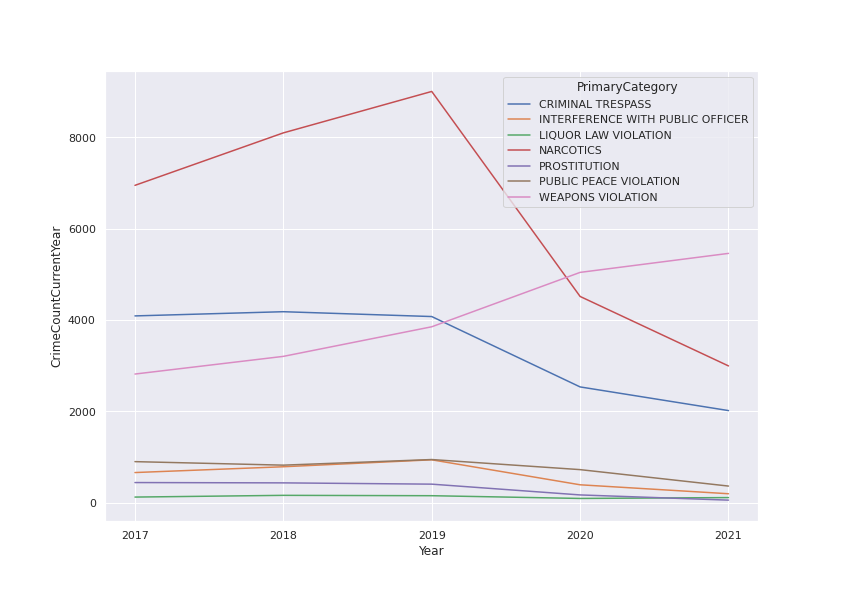
\includegraphics[scale=.3 ]{/home/angelo/Documents/Uni/Courses/Data Managment & Ethics/Integrated Assignment/assignemnet_project_folder/Code/q1_part2.png}
   \caption{Resource intensive Crimes Annual Change}
   \label{fig:Ng2}
\end{subfigure}

\begin{subfigure}[b]{0.5\textwidth}
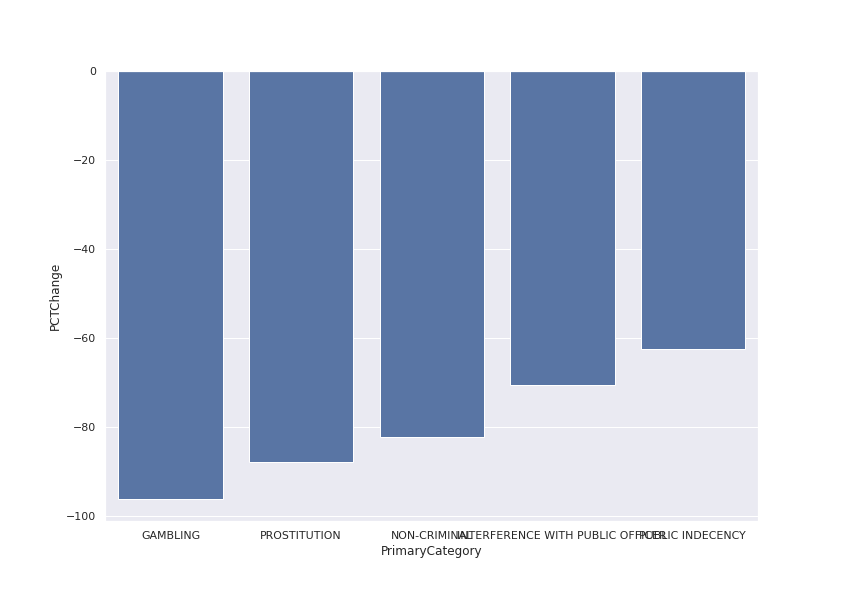
\includegraphics[scale=.3 ]{/home/angelo/Documents/Uni/Courses/Data Managment & Ethics/Integrated Assignment/assignemnet_project_folder/Code/q1_part3a.png}
   \caption{Crime Categories with the greates Reduction}
   \label{fig:Ng2}
\end{subfigure}

\begin{subfigure}[b]{0.5\textwidth}
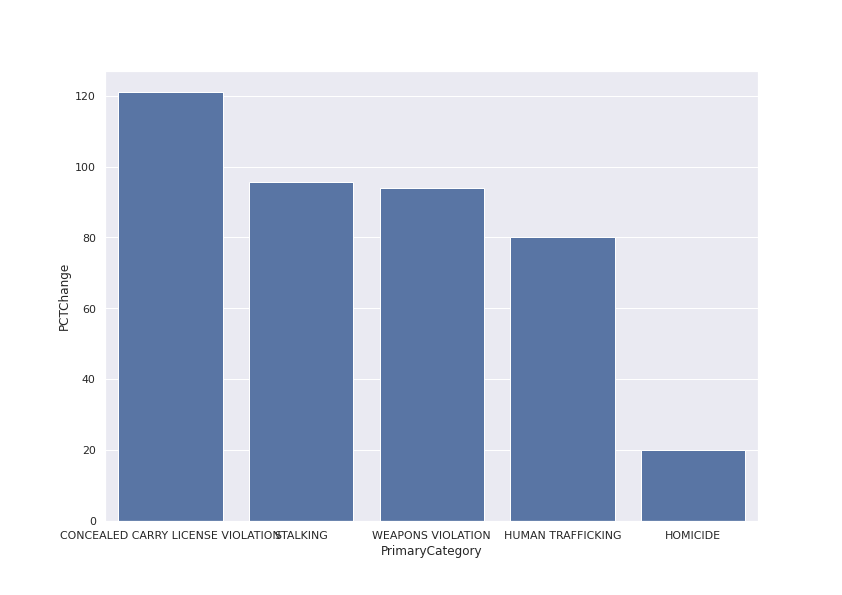
\includegraphics[scale=.3 ]{/home/angelo/Documents/Uni/Courses/Data Managment & Ethics/Integrated Assignment/assignemnet_project_folder/Code/q1_part3b.png}
   \caption{Crime Categories with the greates Increase}
   \label{fig:Ng2}
\end{subfigure}

\captionsetup{justification=centering}
\caption{Temporal Component and Crime by Category}
\end{wrapfigure}



\subsection{Question 2:}

%\begin{itemize}
%  \item Based on overall trends discerned in question 1, what locations (beats \& districts) are disproportinally represented overall and in selected subcategories of crimes (based on Q1)?
%\end{itemize}

When considering the following primary crimetypes 'homicide', 'prostituion', 'weapons violation', 'narcotics' from question 1, these crimes show interestingly large changes to be used as further subsections. Subsequently, question 2 considers which locations are predominant in these crime types. 

After identifying interesting primary types of crimes by time aspect, it is now relevant to subsect the data further by district in order to identify problem districts. To this end, a (large) query was used which uses multiple scalar functions, nested queries and window functions, and a left join plus multiple inner joins and cast functions (this query is too difficult to describe)

The goal was to create a ranking based on the total proportion of the primary category crimes identified ('homicide', 'prostituion', 'weapons violation', 'narcotics') in question 1 per district, limiting the results to the top three districts per crime category. To this end, a (large) query was used which uses multiple scalar functions, nested queries and window functions, and a left join plus multiple inner joins and cast functions (this query is too difficult to describe). It started out in a subquery which calculates the total crimes commited per primary category using two join statements. Next, a subquery was created which also used conventional group statements to calculate the primary crimes committed per district. The first query was then left joined onto the second query, as the first subquery contained only the overall totals per category, which then had to be cast to the dimensions of the second query using a LEFT JOIN. Finally, a $DENSE RANK()$ ranked each priamry category by its proportion in total crimes committed and limited the output to three districts per primary crime category (see Question 2 tab).

Table 1 reports the result of this query.\footnote{see attached python file for stagazer output generation} What is striking (I was surprised myself): in all crime categories that saw the largest movement over the years, district 11 is in at least the top three for each crime category. Consequently, district 11 must be monitored more closely. 

\begin{table}[!htbp] \centering 
\begin{adjustwidth}{1.25cm}{-0cm}
\begin{threeparttable}
\small
\captionsetup{font=small, justification=raggedright,singlelinecheck=false}
\caption{\textsc{Districts Ranked by Proportion of Crimes Committed}}
\centering 
  \label{}
\small 
\begin{tabular}{@{\extracolsep{10pt}}llrrr} 
\\[-5.8ex]\hline 
\hline \\[-1.8ex] 
\toprule
  Prim.Cat. & District &  Rank &  Tot.Crimes District &  PCT of total crimes \\
\midrule
         HOMICIDE &       11 &                     1 &                          211 &                   11.32\% \\
         HOMICIDE &       06 &                     2 &                          178 &                    9.55\% \\
         HOMICIDE &       05 &                     3 &                          153 &                    8.21\% \\
        NARCOTICS &       11 &                     1 &                        10157 &                   32.20\% \\
        NARCOTICS &       10 &                     2 &                         3540 &                   11.22\% \\
        NARCOTICS &       15 &                     3 &                         2194 &                    6.95\% \\
     PROSTITUTION &       11 &                     1 &                          856 &                   57.37\% \\
     PROSTITUTION &       07 &                     2 &                          179 &                   12.00\% \\
     PROSTITUTION &       05 &                     3 &                          132 &                    8.85\% \\
WEAPONS VIOLATION &       07 &                     1 &                         2190 &                   10.76\% \\
WEAPONS VIOLATION &       11 &                     2 &                         2185 &                   10.73\% \\
WEAPONS VIOLATION &       06 &                     3 &                         2023 &                    9.94\% \\
\bottomrule
\hline 
\hline \\[-3.5ex] 
\end{tabular} 
\begin{tablenotes}[para,flushleft]
      \small
      \item\textit{ }
    \end{tablenotes}
\end{threeparttable}
\end{adjustwidth}
%
\end{table}







\subsection{Question 3:}


Finally, based on the trends observed in question 1 and the locations in question 2, we will look at how we can prevent these crimes by allocating resources efficiently to those locations by time of day during time of day (eg morining)


\begin{itemize}
  \item Triangulating time, crime-type, and location which areas persists in certain crimes wrt. time?
In order to prevent homicides; which “beats“ are the most prevalent among homicides? During which time of day (for effective allocation of policing resources)? 
\end{itemize}


%\begin{itemize}
%  \item Triangulating time, crime-type, and location which areas persists in certain crimes wrt. time?
%In order to prevent homicides; which “beats“ are the most prevalent among homicides? During which time of day (for effective allocation of policing resources)? 





\subsection{Conclusion}



















\end{document}
